% Chapter X

\chapter{Progettazione della base di dati spaziale} % Chapter title
I risultati ottenuti dal metodo devono poter essere consultati agevolmente per facilitare le decisioni riguardo 
la prevenzione del territorio. Questa esigenza si traduce nella creazione di una basi di dati geografica che riassume i risultati ottenuti dal metodo. Sfruttando le tecnologie messe a disposizione dai sistemi GIS (Geographical Information System), sarà possibile valutare i risultati presenti nella base di dati attraverso il rendering dei dati su una mappa geografica. Tale visualizzazione contestualizza meglio i risultati rendendoli più chiari. Questa motivazione esprime l'importanza di una base dati. Verrà quindi illustrata la sua progettazione attraverso le tecniche tipiche di questo ambito.


Si è progettata quindi la base di dati seguendo i seguenti passi progettuali.

\begin{figure}[h]
	\centering
	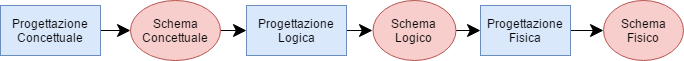
\includegraphics[width=1\textwidth]{images/Progettazione.png}
	\caption{In figura vengono brevemente mostrati i passi concettuali nella progettazione di una base di dati. In blu vengono rappresentate le fasi concettuali. In rosso vengono rappresentati i vari schemi e descrizioni che si acquisiscono in output alla fine di ogni ogni fase progettuale}
	\label{fig:diagrammaER}
\end{figure}

Come primo passo si devono trasporre le definizioni e le notazioni introdotte in concetti propri delle basi di dati.
Definiamo quindi una relazione: 
\begin{enumerate}
	\item geoarea $\leftarrow$ $GEOAREA$
	\item dataset $\leftarrow$ $\mathcal{Z}$
	\item isoipse\_abruzzo\_25 $\leftarrow$ $\mathcal{I}$
	\item raylway\_station $\leftarrow$ $\mathcal{B}$
	\item station\_exposure $\leftarrow$ $\mathcal{EXP}$
	\item railway\_routes $\leftarrow$ $\mathcal{R}$
	\item railway\_routes\_segment $\leftarrow$ $\mathcal{SR}$
	\item segment\_exposure $\leftarrow$ $\mathcal{EXPSR}$
\end{enumerate}
Tale relazione definisce le entità. Esse rappresentano concetti complessi e di rilievo che descrivono classi di oggetti con esistenza autonoma. Un'istanza di un' entità è un oggetto della classe rappresentata. Un'entità ha un nome univoco all'interno dello schema concettuale e viene rappresentata nel diagramma ER con un rettangolo con il nome dell'entità all'interno. \\
Per ogni entità vengono mostrate
\begin{enumerate}
	\item Gli attributi descritti da un pallino vuoto;
	\item L'attributo identificante descritto da un pallino nero pieno;
	\item I vincoli di partecipazione nelle relazioni, con notazione (min,max).
\end{enumerate}


\begin{figure}[h]
	\centering
	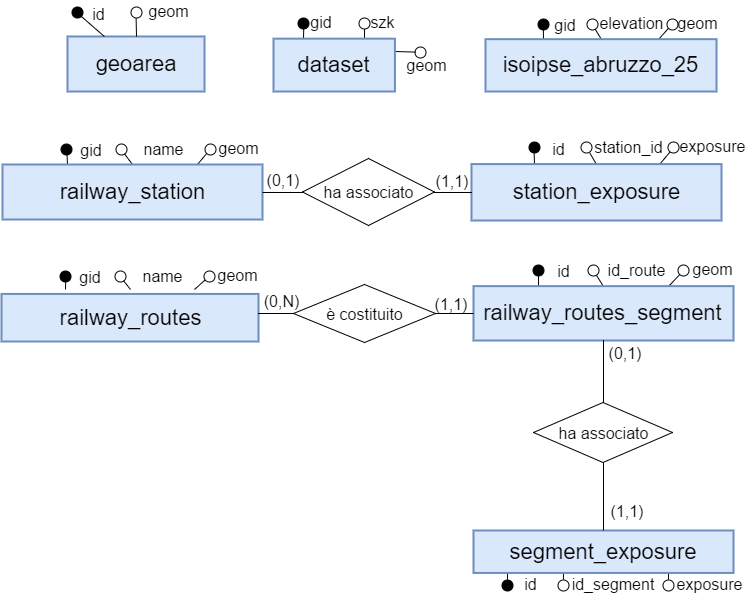
\includegraphics[width=0.9\textwidth]{images/DiagrammaEr.png}
	\caption{In figura è rappresentato il diagramma Er della base di dati. sono presenti 3 associazioni ed 8 entità.}
	\label{fig:diagrammaER}
\end{figure}

\begin{table}[h]
	\centering
	\renewcommand{\arraystretch}{1.4}
	
	\begin{tabular}{|c|c|c|c|}
		\hline
		\rowcolor[HTML]{C0C0C0} 
		Entità                   & Descrizione                                                                                                                                                 & Attributi                                                           & Attributi Identificanti \\ \hline
		\multicolumn{1}{|l|}{}   & \multicolumn{1}{l|}{}                                                                                                                                       & \multicolumn{1}{l|}{}                                               & \multicolumn{1}{l|}{}   \\ \hline
		geoarea                  & \begin{tabular}[c]{@{}c@{}}Entità relativa al territorio \\ di interesse, nel nostro caso la \\ regione Abruzzo\end{tabular}                                & \begin{tabular}[c]{@{}c@{}}id\\ geom\end{tabular}                   & id                      \\ \hline
		dataset                  & \begin{tabular}[c]{@{}c@{}}Entità relativa al territorio \\ partizionato della regione abruzzo\end{tabular}                                                 & \begin{tabular}[c]{@{}c@{}}gid \\ szk\\ geom\end{tabular}           & gid                     \\ \hline
		isoipse\_abruzzo\_25     & \begin{tabular}[c]{@{}c@{}}Entità relativa alle isoipse contenute \\ all'interno del territorio abruzzese.\end{tabular}                                     & \begin{tabular}[c]{@{}c@{}}gid \\ elevation\\ geom\end{tabular}     & gid                     \\ \hline
		railway\_station         & \begin{tabular}[c]{@{}c@{}}Entità relativa alle stazioni presenti \\ sul suolo della regione di interesse\end{tabular}                                      & \begin{tabular}[c]{@{}c@{}}gid \\ name\\ geom\end{tabular}          & gid                     \\ \hline
		station\_exposure        & \begin{tabular}[c]{@{}c@{}}Entità relativa all'esposizione al rischio \\ frana da parte di una stazione\end{tabular}                                        & \begin{tabular}[c]{@{}c@{}}id\\ station\_id\\ exposure\end{tabular} & id                      \\ \hline
		railway\_routes          & \begin{tabular}[c]{@{}c@{}}Entità relativa alle linee ferroviarie della\\ regione di interesse\end{tabular}                                                 & \begin{tabular}[c]{@{}c@{}}gid\\ name \\ geom\end{tabular}          & gid                     \\ \hline
		railway\_routes\_segment & \begin{tabular}[c]{@{}c@{}}Entità relativa ai vari segmenti che \\ compongono le linee ferroviarie\end{tabular}                                             & \begin{tabular}[c]{@{}c@{}}id\\ id\_route\\ geom\end{tabular}       & id                      \\ \hline
		segment\_exposure        & \begin{tabular}[c]{@{}c@{}}Entità relativa all'esposizione al rischio \\ di frana da parte di un segmento che \\ compone una linea ferroviaria\end{tabular} & \begin{tabular}[c]{@{}c@{}}id\\ id\_segment\\ exposure\end{tabular} & id                      \\ \hline
	\end{tabular}
	\caption{In tabella sono descritte le entità in modo dettagliato}
	\label{tab:entita}
\end{table}

\begin{table}[h]
	\centering
	\renewcommand{\arraystretch}{1.2}
	\begin{tabular}{|c|c|c|c|}
		\hline
		\rowcolor[HTML]{C0C0C0} 
		Associazione           & Descrizione                                                                                                                                                                                 & Entità coinvolte                                                                                                                                                    & Attributi             \\ \hline
		\multicolumn{1}{|l|}{} & \multicolumn{1}{l|}{}                                                                                                                                                                       & \multicolumn{1}{l|}{}                                                                                                                                               & \multicolumn{1}{l|}{} \\ \hline
		ha associato           & \begin{tabular}[c]{@{}c@{}}La seguente relazione evidenzia che\\ una stazione può avere associato un valore\\ di exposure. Stessa considerazione si può fare \\ per i segmenti\end{tabular} & \begin{tabular}[c]{@{}c@{}}railway\_station\textless\textgreater      station\_exposure\\ railway\_routes\_segment\textless\textgreater segment\_exposure\end{tabular} & nessuno               \\ \hline
		è costituito           & \begin{tabular}[c]{@{}c@{}}La seguente relazione evidenzia che una route \\ può essere associata con N segmenti. Un segmento\\ può appartenere ad una sola route\end{tabular}               & railway\_routes\textless\textgreater railway\_routes\_segment                                                                                                      & nessuno               \\ \hline
	\end{tabular}
	\caption{tab:associazioni}
	\label{In tabella sono descritte le associazioni in modo dettagliato}
\end{table}

Dallo schema Concettuale si è progettato quello logico nel seguente modo.

\begin{enumerate}
	\item geoarea(\underline{id},geom)
	\item dataset(\underline{gid},szk,geom) 
	\item isoipse\_abruzzo\_25(\underline{gid},elevation,geom)
	\item railway\_station(\underline{gid},name,geom)
	\item station\_exposure(\underline{id},station\_id,exposure)
	\begin{enumerate}
		\item FK: station\_id REFERENCES railway\_station  
	\end{enumerate}
	\item railway\_routes(\underline{gid},name,geom)
	\item railway\_routes\_segment(\underline{id},id\_route,geom)
	\begin{enumerate}
		\item FK: id\_route REFERENCES railway\_routes
	\end{enumerate}
	\item segment\_exposure(\underline{id},id\_segment,exposure)
	\begin{enumerate}
		\item FK: id\_segment REFERENCES railway\_routes\_segment
	\end{enumerate}
\end{enumerate}

Per quanto riguarda lo schema fisico esso verrà esposto in appendice.
